\documentclass[conference]{IEEEtran}
\usepackage[T1]{fontenc}
\usepackage{newtxtext,newtxmath}
\usepackage{amsmath}
\usepackage{graphicx}
\usepackage{booktabs}
\usepackage{siunitx}
\usepackage[hidelinks]{hyperref}
\graphicspath{{phase1/figures/}{data/figures/}}
\sisetup{group-minimum-digits=4}

% house style: no em dashes, so the abstract heading uses a colon
\makeatletter
\def\abstract{\normalfont\@IEEEabskeysecsize\bfseries\textit{\abstractname}:\ \relax\@IEEEgobbleleadPARNLSP}
\makeatother

\newcommand{\ugm}{\si{\micro\gram\per\cubic\metre}}
\newcommand{\col}[1]{\texttt{#1}}

% allow more floats per page so tables and figures stay near their text
\renewcommand{\topfraction}{0.85}
\renewcommand{\bottomfraction}{0.6}
\renewcommand{\textfraction}{0.1}
\renewcommand{\floatpagefraction}{0.75}
\setcounter{topnumber}{3}
\setcounter{bottomnumber}{2}
\setcounter{totalnumber}{5}

\begin{document}

\title{Six-hour PM2.5 forecasting in Beijing with gradient boosting and leak-free testing}

\author{\IEEEauthorblockN{Vetriselvan R, Hrishi Dongre, Pampana Sree Adithya, Ishan Goyal, Vedant Madne}
\IEEEauthorblockA{Team T024, Section A - AML/DL Project 19: Air quality forecasting via gradient boosting and LSTM models}}

\maketitle

\begin{abstract}
We forecast hourly PM2.5 at the US Embassy in Beijing six hours ahead, using only what is known when the forecast is made. The model sees 52 inputs: PM2.5 history, rolling statistics, the calendar, weather from the hour before, derived weather, and four physics inputs for still air, southerly wind and humidity taken from research on Beijing smog. XGBoost, averaged over five seeds, is blended with ridge regression. Every setting is chosen on the validation years 2011 to 2013, and each final model is scored once on the test year 2014. On 2014 the blend reaches RMSE 51.96~\ugm, MAE 33.93 and $R^2$ 0.690, against 61.22, 38.67 and 0.569 for the forecast ``no change'' (persistence): 15.1\% lower RMSE. A mixture of experts that adds a spike expert for hours above 150~\ugm{} is our final model: RMSE 51.86, MAE 33.69 and $R^2$ 0.691 on 2014. Most of the remaining error sits in the start and end of smog episodes.
\end{abstract}

\section{Introduction}
Beijing's PM2.5 swings between clean air and severe smog that lasts for days \cite{liang2015}. A forecast a few hours ahead supports health warnings, but it is only useful if it beats the simplest rule, that PM2.5 stays at its current value (persistence), and if it is tested on data the model has never seen.

We use the UCI Beijing PM2.5 dataset \cite{uci}. This report covers Phase 1, gradient boosting; Phase 2 will use deep learning. A companion report \cite{datareport} covers the exploratory data analysis (EDA) and preprocessing. We fixed six hours as the target before building any model: on 2010 to 2013, ``no change'' misses by only 13.1~\ugm{} on average one hour ahead, which is too easy to improve on, and by 69.8 a day ahead, where little of the past still helps. Six hours (40.8) is the useful middle.

Our contributions are:
\begin{itemize}
\item a leak-free setup: training only on earlier years, a one-day gap before each evaluation year, and a test year that each model may be scored on only once (Section~\ref{sec:protocol});
\item physics inputs from smog research, and tests of what each feature group adds (Sections~\ref{sec:features} and \ref{sec:results});
\item an XGBoost and ridge blend that beats persistence by 15.1\% RMSE on the unseen year 2014, and a mixture of experts that lowers MAE further (Sections~\ref{sec:results} and \ref{sec:moe}).
\end{itemize}

\section{Related work}
\label{sec:related}
\textbf{Beijing smog.} Liang et al. \cite{liang2015} introduced our dataset and showed that weather explains much of the variation in Beijing's PM2.5. Zhong et al. \cite{zhong2018} describe winter episodes in two stages: pollution first blows in on southerly winds, then piles up under calm, humid air. Huang et al. \cite{huang2018} review the air stagnation index, which calls the air stagnant when the surface wind is below 3.2~m/s, the upper-level wind is weak and no rain falls. Our physics inputs come from these two papers.

\textbf{Models.} Persistence and the same hour one day earlier (seasonal-naive) are the standard simple forecasts to beat \cite{hyndman2021}. Ridge regression \cite{hoerl1970} is a linear model with a penalty that keeps its weights stable when inputs move together. XGBoost \cite{chen2016} adds many small regression trees and handles non-linear effects and mixed scales without preprocessing. Recurrent networks such as the LSTM \cite{hochreiter1997} are our Phase 2 candidates. A mixture of experts \cite{jacobs1991} lets a gate decide, input by input, how much to trust each expert model.

\textbf{Benchmark.} Wang and Du \cite{wang2026} compare the same model types on 12 Beijing stations (2013 to 2017) with extra pollutants such as PM10 as inputs. Their best $R^2$ six hours ahead is 0.660, with XGBoost best at that horizon.

\textbf{Leakage.} Using information a model would not have at prediction time inflates scores \cite{kaufman2012}. Our rules against it are in Section~\ref{sec:protocol}.

\section{Data and what the EDA showed}
\label{sec:data}
The dataset \cite{uci} has hourly PM2.5 from the US Embassy and weather from Beijing Capital International Airport, from 1 January 2010 to 31 December 2014 (\num{43824} hours, none skipped). Only PM2.5 has gaps: \num{2067} hours, 4.72\%. The wind speed column is a running total and is decoded into hourly speed \cite{datareport}. The years 2010 to 2013 are used to build the models and 2014 is kept for the final test. Table~\ref{tab:eda} lists the EDA findings, all from 2010 to 2013, and what each one changed in the model.

\begin{table}[!htb]
\centering
\caption{EDA findings on 2010 to 2013 and what they changed \cite{datareport}}
\label{tab:eda}
\begin{tabular}{@{}p{0.52\columnwidth}p{0.40\columnwidth}@{}}
\toprule
Finding & What the model gets \\
\midrule
``No change'' misses by 13.1, 40.8 and 69.8~\ugm{} at 1, 6 and 24 h & Six-hour target; past PM2.5 and rolling averages \\
PM2.5 peaks at 21:00 in winter and at 08:00 in summer & Hour and month of the target hour \\
North-west wind is cleanest (median 31), calm and south-east wind dirtiest (100 and 93) & Wind direction and a north-west wind total \\
Humid air goes with dirtier air (rank correlation 0.54) & Humidity and humid hours \\
322 episodes of 6 or more hours above 150~\ugm: they build over about 55 hours and clear in about 14 & Physics inputs; a separate score above 150 \\
Lunar New Year fireworks reach 7 to 14 times the usual level & A New Year flag \\
\bottomrule
\end{tabular}
\end{table}

\begin{figure}[!t]
\centering
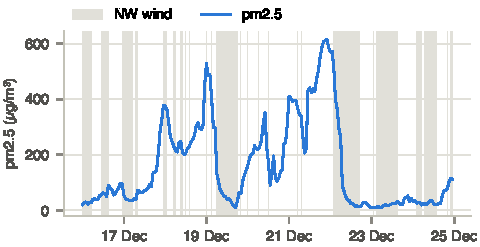
\includegraphics[width=\columnwidth]{episode.pdf}
\caption{Two episodes in December 2010: a slow build-up, then a collapse when steady north-west wind (shaded) arrives \cite{datareport}.}
\label{fig:episode}
\end{figure}

\section{Setup and fair testing}
\label{sec:protocol}

\subsection{What the model sees}
Let $y_t$ be PM2.5 at hour $t$, the moment the forecast is made. One model predicts six hours ahead directly,
\begin{equation}
\hat{y}_{t+6} = f(\mathbf{x}_t),
\end{equation}
where $\mathbf{x}_t$ holds PM2.5 up to hour $t$, weather up to hour $t-1$, and the calendar of the target hour $t+6$, which is known in advance. Weather is taken one hour early as a safety margin: another UCI release of the same station \cite{fivecities} has the same weather but PM2.5 shifted by one hour, and we cannot tell which clock is right. Missing PM2.5 inputs repeat the last known value for at most three hours; the value a model is scored against is never filled.

\subsection{Folds and test year}
The data are split by year (Fig.~\ref{fig:folds}; the code calls the folds cv1 to cv3). Fold 1 trains on 2010 and is validated on 2011; fold 2 trains on 2010 and 2011 and is validated on 2012; fold 3 trains on 2010 to 2012 and is validated on 2013. A 24-hour gap before each evaluation year keeps its answers out of training, and an hour is scored only if its forecast time and its target are both inside the evaluation year. A code review on 19 October 2026, before the first model run, found that this last rule was missing: forecasts made in the last six hours of 2013 would have been checked against PM2.5 values from 2014, the test year. We fixed it and added tests before any model was trained, so no reported score was affected. All settings are chosen on these three validation years, \num{24417} hours in total, the same hours for every model. The final models train on 2010 to 2013 and are tested on 2014.

\begin{figure}[!t]
\centering
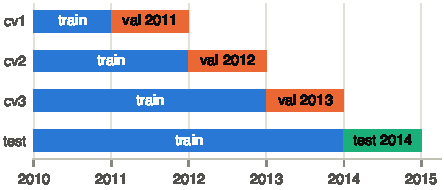
\includegraphics[width=\columnwidth]{folds.pdf}
\caption{Folds cv1 to cv3 and the test fold: each trains on earlier years only \cite{datareport}.}
\label{fig:folds}
\end{figure}

Each model may be scored on 2014 only once. The test code stops if test scores already exist and stores a fingerprint of the settings it used. The Phase 1 blend was scored on 19 October 2026. The mixture of experts (Section~\ref{sec:moe}) was chosen as the final model on the validation years, and that choice was committed to the repository before it was scored on 2014 on 25 October 2026. No setting was chosen from a test score. Twenty-two automated tests check the pipeline and these rules, for example that cutting the data at an hour leaves every input before the cut unchanged.

\subsection{Scores}
With errors $e_i = \hat{y}_i - y_i$ over $n$ hours,
\begin{gather}
\text{MAE} = \frac{1}{n}\sum_i |e_i|, \qquad \text{RMSE} = \sqrt{\frac{1}{n}\sum_i e_i^2}, \\
R^2 = 1 - \frac{\sum_i e_i^2}{\sum_i (y_i - \bar{y})^2}, \qquad \text{skill} = 1 - \frac{\text{RMSE}}{\text{RMSE}_{\text{persistence}}}.
\end{gather}
MAE is the average miss in \ugm, RMSE weighs big misses more, $R^2$ is the share of the variation the forecast explains, and skill is how much lower the RMSE is than that of ``no change'' on the same hours. Settings are chosen by RMSE, the error both models train on.

\section{Features}
\label{sec:features}
Table~\ref{tab:features} lists the 52 inputs. One of them, \col{pm\_anom}, is PM2.5 now minus the usual PM2.5 for that hour of day in the training years, so it says how unusual the current level is.

\begin{table}[!htb]
\centering
\caption{The 52 inputs in six groups}
\label{tab:features}
\begin{tabular}{@{}lrp{0.62\columnwidth}@{}}
\toprule
Group & $n$ & Inputs \\
\midrule
Lags & 10 & PM2.5 now and 1, 2, 3, 6, 12, 24, 48 h ago; missing flag; missing hours in the last day \\
Rolling & 15 & mean, spread and max over 3, 6, 12, 24 h; change over 1 and 3 h; \col{pm\_anom} \\
Calendar & 7 & hour and month of the target hour (as sine and cosine), day of week, weekend, Lunar New Year \\
Weather & 11 & dew point, temperature, pressure, wind speed, running wind total, rain, snow, four wind directions, all from hour $t-1$ \\
Derived & 5 & humidity, pressure change over 3 and 24 h, hours the wind has kept its direction, north-west wind over 24 h \\
Physics & 4 & still hours in the last day, current still run, south-east wind over 24 h, humid hours in the last day \\
\bottomrule
\end{tabular}
\end{table}

The physics inputs turn the smog research into hourly numbers. An hour counts as still when the wind is weak and no rain falls,
\begin{equation}
s_t = 1 \text{ if } ws_t < 3.2\ \text{m/s and no rain, else } 0,
\end{equation}
the ground-level part of the stagnation index \cite{huang2018}. From it, \col{stag24} counts the still hours in the last 24 and \col{stag\_run} is how long the air has been still. \col{se\_ws24} adds up south-east wind speed over 24 hours, our stand-in for the southerly winds of \cite{zhong2018} because the data have no south-west direction, and \col{humid24} counts hours above 80\% humidity. A tree looks at one hour at a time and cannot count hours by itself, so these inputs give it a memory of the last day.

\section{Models}
\label{sec:models}

\subsection{Baselines}
Persistence forecasts $\hat{y}_{t+6} = y_t$ (``no change''). Seasonal-naive forecasts the value at the same hour one day earlier.

\subsection{Ridge regression}
Ridge \cite{hoerl1970} finds the weights $\boldsymbol{\beta}$ that minimise
\begin{equation}
\sum_i (y_i - \mathbf{x}_i^\top\boldsymbol{\beta})^2 + \alpha \lVert\boldsymbol{\beta}\rVert^2 .
\end{equation}
The penalty $\alpha$ keeps the weights small and stable when inputs move together, as dew point, temperature and pressure do. Inputs are standardised using the training years only. Validation chose $\alpha = 10$ from $\{0.1, 1, 10, 100, 1000\}$.

\subsection{XGBoost}
XGBoost \cite{chen2016} builds the forecast as a sum of regression trees, each a set of yes/no questions on the inputs that ends in a number. Trees are added one at a time, each fitted to what the previous ones still get wrong, to minimise
\begin{equation}
\mathcal{L} = \sum_i \tfrac{1}{2}(y_i - \hat{y}_i)^2 + \sum_{\text{trees}} \tfrac{1}{2}\lambda \lVert \mathbf{w}\rVert^2 ,
\end{equation}
where $\mathbf{w}$ are the leaf values and $\lambda$ is an L2 (ridge) penalty on them. For squared error, the value of leaf $j$ is
\begin{equation}
w_j = \frac{\sum_{i \in j} (y_i - \hat{y}_i)}{n_j + \lambda},
\end{equation}
the sum of the current misses of the $n_j$ training hours in that leaf, shrunk by $\lambda$, and each tree adds it scaled by the learning rate 0.05. The trees ask whichever questions lower the error most; we only choose the inputs and the limits.

A random search tried 20 settings on the validation years. It chose trees of depth 4, at least 20 hours per leaf, half the inputs per tree and $\lambda = 1$. Each fit uses the last 90 training days to decide when to stop adding trees (about 127 on average) and is then refitted on all training hours. The final forecast averages five models with different random seeds.

\subsection{Blend and target}
The blend is 0.6~$\times$~XGBoost~$+$~0.4~$\times$~ridge, with weights chosen on a 0.1 grid by validation RMSE. Both models predict PM2.5 directly. Predicting $\log(1 + y)$ instead made XGBoost's forecasts 12.6~\ugm{} too low on average (RMSE 59.96 against 56.81), so we kept the raw value.

\section{Results}
\label{sec:results}
Table~\ref{tab:results} shows the six-hour scores. On validation and on 2014, the blend beats both baselines and both of its parts on RMSE and $R^2$, and the mixture of experts (Section~\ref{sec:moe}) is a little better again on MAE.

\begin{table}[!htb]
\centering
\caption{Six-hour scores. Validation: 2011 to 2013, used for every choice. Test: 2014, scored once per model. RMSE and MAE in \ugm.}
\label{tab:results}
\setlength{\tabcolsep}{4pt}
\begin{tabular}{@{}lrrrr@{}}
\toprule
Model & RMSE & MAE & $R^2$ & Skill \\
\midrule
\multicolumn{5}{@{}l}{\textit{Validation, 2011 to 2013}} \\
Persistence & 65.77 & 40.23 & 0.483 & 0.0\% \\
Seasonal-naive & 101.42 & 69.42 & $-$0.230 & $-$54.2\% \\
Ridge & 57.66 & 38.27 & 0.602 & 12.3\% \\
XGBoost (5 seeds) & 56.81 & 36.46 & 0.614 & 13.6\% \\
Blend & 56.33 & 36.41 & 0.621 & 14.4\% \\
Mixture of experts & \textbf{56.26} & \textbf{35.99} & \textbf{0.622} & \textbf{14.5\%} \\
\midrule
\multicolumn{5}{@{}l}{\textit{Test, 2014}} \\
Persistence & 61.22 & 38.67 & 0.569 & 0.0\% \\
Seasonal-naive & 98.74 & 67.30 & $-$0.121 & $-$61.3\% \\
Ridge & 54.20 & 36.11 & 0.662 & 11.5\% \\
XGBoost (5 seeds) & 52.21 & 33.79 & 0.687 & 14.7\% \\
Blend & 51.96 & 33.93 & 0.690 & 15.1\% \\
Mixture of experts & \textbf{51.86} & \textbf{33.69} & \textbf{0.691} & \textbf{15.3\%} \\
\bottomrule
\end{tabular}
\end{table}

\subsection{How the model improved}
Table~\ref{tab:runs} shows the six-hour model step by step. The first version predicted $\log(1 + y)$ and chose settings by MAE; undoing the log made its forecasts 12.7~\ugm{} too low on average. Predicting PM2.5 directly gave the largest gain. Choosing every setting by RMSE and adding the physics inputs gave the final blend.

\begin{table}[!htb]
\centering
\caption{How the six-hour model improved. Skill: how much smaller the RMSE is than that of ``no change''}
\label{tab:runs}
\setlength{\tabcolsep}{4pt}
\begin{tabular}{@{}llrr@{}}
\toprule
Step & Change & RMSE & Skill \\
\midrule
Run 1 & first version, log target & 59.70 & 9.2\% \\
Run 2 & predict PM2.5 directly & 56.69 & 13.8\% \\
Runs 3 and 4 & physics inputs, tuned by RMSE & 56.33 & 14.4\% \\
Blend, 2014 & scored once & 51.96 & 15.1\% \\
Mixture, 2014 & final model, scored once & 51.86 & 15.3\% \\
\bottomrule
\end{tabular}
\end{table}

\subsection{Did it carry over to 2014?}
Yes. 2014 is an easier year (persistence explains 56.9\% of the variation against 48.3\% on validation), so errors are lower everywhere and the fair comparison is skill: 15.1\% on 2014 against 14.4\% on validation for the blend. Our $R^2$ of 0.690 is close to the 0.660 of the 12-station benchmark \cite{wang2026}; the data differ, so this shows the problem is similar, not that one model is better.

\subsection{Why six hours}
Fig.~\ref{fig:horizon} repeats the forecast at other horizons. At one hour persistence already explains 93\% of the variation, so a model adds little; at 12 hours XGBoost explains only 36.5\%. Six hours is the longest tested horizon at which the model explains most of the variation (0.614) while clearly beating persistence.

\begin{figure}[!t]
\centering
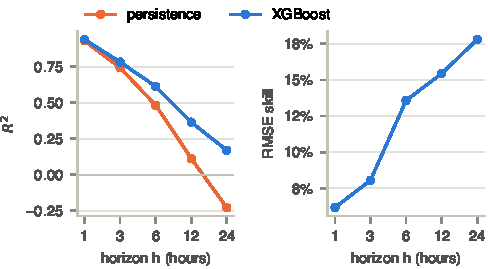
\includegraphics[width=\columnwidth]{horizon.pdf}
\caption{Validation $R^2$ of persistence and XGBoost (left) and XGBoost skill (right) by horizon, one seed.}
\label{fig:horizon}
\end{figure}

\subsection{What each feature group adds}
Fig.~\ref{fig:ablation} adds the feature groups one at a time, five seeds per point. PM2.5 history alone gives RMSE 62.05. Every group lowers the error; weather gives the largest drop (60.16 to 58.02), and the physics group lowers it from 57.17 to 56.81.

\begin{figure}[!t]
\centering
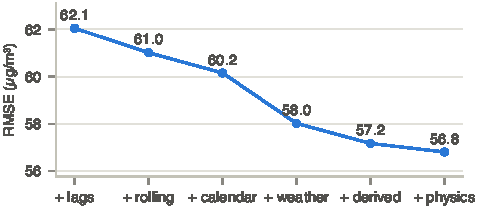
\includegraphics[width=\columnwidth]{ablation.pdf}
\caption{Validation RMSE at six hours as feature groups are added (XGBoost, mean of 5 seeds).}
\label{fig:ablation}
\end{figure}

\subsection{Which inputs matter most}
Table~\ref{tab:importance} uses permutation importance \cite{breiman2001}: shuffle one input on the evaluation year, so it no longer lines up with the right hours, and measure how much RMSE rises (mean of five shuffles, one model trained on 2010 to 2012 and evaluated on 2013). Two physics inputs rank 3rd and 6th of 52, ahead of every raw weather reading.

\begin{table}[!htb]
\centering
\caption{Top 8 inputs: RMSE rise when shuffled (\ugm)}
\label{tab:importance}
\begin{tabular}{@{}llr@{}}
\toprule
Input & Group & RMSE rise \\
\midrule
\col{pm\_anom} (how unusual PM2.5 is now) & rolling & 19.32 \\
\col{pm\_0} (PM2.5 now) & lags & 2.35 \\
\col{stag\_run} (still-air run) & physics & 1.95 \\
\col{hour\_cos} (hour of day) & calendar & 1.65 \\
\col{pm\_mean24} (24 h average) & rolling & 1.49 \\
\col{stag24} (still hours) & physics & 1.39 \\
\col{pres\_diff3} (3 h pressure change) & derived & 1.11 \\
\col{wd\_se} (south-east wind) & weather & 1.04 \\
\bottomrule
\end{tabular}
\end{table}

\subsection{Training against validation}
Table~\ref{tab:trainval} puts each model's score on the hours it trained on next to its validation score, averaged over the three folds, to read bias and variance.

\begin{table}[!htb]
\centering
\caption{Training against validation, mean of the three folds}
\label{tab:trainval}
\setlength{\tabcolsep}{4pt}
\begin{tabular}{@{}lrrrr@{}}
\toprule
 & \multicolumn{2}{c}{$R^2$} & \multicolumn{2}{c}{RMSE (\ugm)} \\
\cmidrule(lr){2-3}\cmidrule(l){4-5}
Model & train & validation & train & validation \\
\midrule
Persistence & 0.439 & 0.475 & 68.63 & 65.59 \\
Blend & 0.694 & 0.614 & 50.71 & 56.20 \\
Mixture of experts & 0.721 & 0.615 & 48.34 & 56.12 \\
\bottomrule
\end{tabular}
\end{table}

Even on its own training hours the blend explains only about 69\% of the variation, so the main limit is information, not overfitting: the inputs at hour $t$ cannot tell what the weather will do in the next six hours. The gap to validation (about 0.08 in $R^2$) shows moderate variance, and part of it is simply that every validation year is a new year. The models trained on 2010 to 2013 agree: training $R^2$ 0.724 for the blend and 0.737 for the mixture, against 0.690 and 0.691 on 2014.

\subsection{Where the errors are}
Winter is the hardest season (blend RMSE 75.57 against 45.08 in spring). Hours whose target is above 150~\ugm{} are 21.2\% of validation hours but carry 50.6\% of the squared error, and the blend predicts them 55.3~\ugm{} too low on average. Fig.~\ref{fig:window} shows the typical failure: the blend follows the build-up but lags the sharp rises and clearings.

\begin{figure}[!t]
\centering
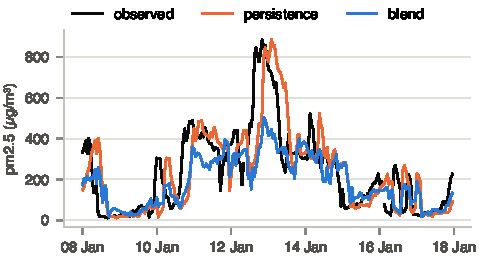
\includegraphics[width=\columnwidth]{window.pdf}
\caption{Six-hour forecasts in January 2013 (a validation year), plotted at their target time.}
\label{fig:window}
\end{figure}

\section{Final model: mixture of experts}
\label{sec:moe}
Because the blend misses the high hours, we gave them their own model. A mixture of experts \cite{jacobs1991} has three parts, all using the same 52 inputs:
\begin{itemize}
\item a quiet expert, the blend recipe trained only on hours whose target is at or below 150~\ugm;
\item a spike expert, XGBoost trained only on hours above 150;
\item a gate, an XGBoost classifier that gives $p$, the chance that PM2.5 six hours later is above 150.
\end{itemize}
The forecast mixes the two experts by that chance:
\begin{equation}
\hat{y} = (1-p)\,\hat{y}_{\text{quiet}} + p\,\hat{y}_{\text{spike}} .
\end{equation}

\begin{table}[!htb]
\centering
\caption{Mixture of experts at six hours, validation years (\ugm)}
\label{tab:moe}
\begin{tabular}{@{}lrr@{}}
\toprule
Model & RMSE & MAE \\
\midrule
Blend & 56.33 & 36.41 \\
Mixture of experts & 56.26 & 35.99 \\
Mixture with a perfect gate (reference) & 39.46 & 27.29 \\
\bottomrule
\end{tabular}
\end{table}

On validation (Table~\ref{tab:moe}) the mixture lowers MAE from 36.41 to 35.99. Rebuilt with three different sets of five seeds, the MAE gain is 0.42 to 0.46 each time while the blend itself moves by only 0.05, so the gain is real. The RMSE gain (0.01 to 0.20) is no larger than the blend's own seed variation (0.12), so RMSE is level. The gate separates high hours well (AUC 0.923), but it struggles to see an episode end: among hours that start above 150, its AUC is 0.734. If the gate knew the true answer, the same experts would cut RMSE by 30\% to 39.46. This is a reference, not a forecast, but it shows the gate is the part to improve.

We fixed the mixture as the final model on this validation evidence and committed that choice before scoring it on 2014. Trained on 2010 to 2013 and scored once, it reaches RMSE 51.86, MAE 33.69 and $R^2$ 0.691, against 51.96, 33.93 and 0.690 for the blend: 0.7\% lower MAE, with RMSE level within seed noise.

\section{Limitations}
\begin{itemize}
\item The data come from one station, without PM10, other pollutants or boundary-layer height.
\item Weather is used one hour late because of the unresolved clock offset; if the clocks agree, this may cost some accuracy.
\item Validation scores are slightly optimistic because settings were chosen on them. 2014 is a single, easier test year, and it has now scored two models, each fixed beforehand.
\item The gate sees the same inputs as the experts, which limits how much the mixture can add.
\end{itemize}

\section{Conclusion and Phase 2}
Using only what is known at the forecast time, our models forecast PM2.5 six hours ahead with 15.1\% lower RMSE than persistence on the unseen year 2014, and the final mixture of experts reaches 15.3\% with a lower MAE. The physics inputs from smog research rank among the most useful inputs. The remaining error is in the start and end of smog episodes, where a perfect gate would cut RMSE by 30\%. Phase 2 will train an LSTM or temporal CNN with the same folds and rules, and test whether a model that reads a longer history can see episodes start and end. Because 2014 has now scored two models, Phase 2 models will be reported on the validation years or tested once on a new year.

\section*{Reproducibility}
The code is at \url{https://github.com/Vetri-78640/aml_dl_pm2.5}: a Python package (\texttt{src/aqf}) for data, features, models and metrics; three configuration files; five notebooks (01 EDA, 02 preprocessing, 03 Phase 1 models, 04 mixture of experts, 05 training against validation); and 22 automated tests. Scores are saved as CSV files and settings and test fingerprints as JSON under \texttt{reports/}.

\section*{Team contributions}
\begin{itemize}
\item \textbf{Vetriselvan R}: project setup and README, Phase 1 experiments, the smog research behind the physics inputs, and the mixture of experts (gate, notebook 04, final model and its 2014 test, model history).
\item \textbf{Hrishi Dongre}: baselines, ridge and XGBoost models, notebook 03 with the Phase 1 experiments and 2014 test, report figures, this report, and notebook 05 (training against validation).
\item \textbf{Pampana Sree Adithya}: preprocessing report and figures, skew check on 2010 to 2013, calendar, humidity and causal feature builders, and the README model diagrams.
\item \textbf{Ishan Goyal}: EDA on the original data (notebook 01), the combined data report, and notebook and README updates.
\item \textbf{Vedant Madne}: preprocessing pipeline and walkthrough (notebook 02), the physics feature code, data and feature tests, and the data folder guides.
\end{itemize}

\begin{thebibliography}{99}
\bibitem{uci} S. Chen, ``Beijing PM2.5,'' UCI Machine Learning Repository, 2015, doi: 10.24432/C5JS49.
\bibitem{liang2015} X. Liang, T. Zou, B. Guo, S. Li, H. Zhang, S. Zhang, H. Huang, and S. X. Chen, ``Assessing Beijing's PM2.5 pollution: severity, weather impact, APEC and winter heating,'' \emph{Proc. R. Soc. A}, vol. 471, no. 2182, Art. no. 20150257, 2015.
\bibitem{datareport} Vetriselvan R, H. Dongre, P. S. Adithya, I. Goyal, and V. Madne, ``Data understanding and leak-free preprocessing for short-horizon PM2.5 forecasting in Beijing,'' Team T024 project report, 2026.
\bibitem{fivecities} S. Chen, ``PM2.5 data of five Chinese cities,'' UCI Machine Learning Repository, 2016, doi: 10.24432/C52K58.
\bibitem{zhong2018} J. Zhong, X. Zhang, Y. Dong, Y. Wang, C. Liu, J. Wang, Y. Zhang, and H. Che, ``Feedback effects of boundary-layer meteorological factors on cumulative explosive growth of PM2.5 during winter heavy pollution episodes in Beijing from 2013 to 2016,'' \emph{Atmos. Chem. Phys.}, vol. 18, pp. 247--258, 2018, doi: 10.5194/acp-18-247-2018.
\bibitem{huang2018} Q. Huang, X. Cai, J. Wang, Y. Song, and T. Zhu, ``Climatological study of the Boundary-layer air Stagnation Index for China and its relationship with air pollution,'' \emph{Atmos. Chem. Phys.}, vol. 18, pp. 7573--7593, 2018, doi: 10.5194/acp-18-7573-2018.
\bibitem{hyndman2021} R. J. Hyndman and G. Athanasopoulos, \emph{Forecasting: Principles and Practice}, 3rd ed. Melbourne, Australia: OTexts, 2021.
\bibitem{hoerl1970} A. E. Hoerl and R. W. Kennard, ``Ridge regression: Biased estimation for nonorthogonal problems,'' \emph{Technometrics}, vol. 12, no. 1, pp. 55--67, 1970.
\bibitem{chen2016} T. Chen and C. Guestrin, ``XGBoost: A scalable tree boosting system,'' in \emph{Proc. 22nd ACM SIGKDD Int. Conf. Knowledge Discovery and Data Mining}, 2016, pp. 785--794, doi: 10.1145/2939672.2939785.
\bibitem{hochreiter1997} S. Hochreiter and J. Schmidhuber, ``Long short-term memory,'' \emph{Neural Computation}, vol. 9, no. 8, pp. 1735--1780, 1997.
\bibitem{jacobs1991} R. A. Jacobs, M. I. Jordan, S. J. Nowlan, and G. E. Hinton, ``Adaptive mixtures of local experts,'' \emph{Neural Computation}, vol. 3, no. 1, pp. 79--87, 1991.
\bibitem{wang2026} Y. Wang and R. Du, ``Same-hour estimation and multi-horizon forecasting of PM2.5 in Beijing: Model comparison and feature-group contributions,'' arXiv:2607.07279v3 [stat.AP], Aug. 2026.
\bibitem{kaufman2012} S. Kaufman, S. Rosset, C. Perlich, and O. Stitelman, ``Leakage in data mining: Formulation, detection, and avoidance,'' \emph{ACM Trans. Knowl. Discov. Data}, vol. 6, no. 4, Art. no. 15, 2012.
\bibitem{breiman2001} L. Breiman, ``Random forests,'' \emph{Machine Learning}, vol. 45, no. 1, pp. 5--32, 2001.
\end{thebibliography}

\end{document}
